The addition of partial state significantly changes how query results are
computed by the underlying dataflow system, and the system must ensure that
partial state produces the same results with partial state as it did without.
This chapter demonstrates how partial state is implemented in Noria such that
the overall system maintains the invariants from \S\ref{s:noria:consistency}
(page \pageref{i:no-spurious}) and \S\ref{s:eviction} (page
\pageref{i:missing-suffix}).

The biggest change that partial state introduces is that multiple updates may
now be collapsed and re-processed through the dataflow as a single, consolidated
update in response to an upquery. These consolidated updates represent snapshots
of upstream state, and Noria must ensure that these snapshots do not cause reads
to violate any of the system invariants. In particular, Noria must ensure that
the upquery responses indeed represent a particular point in time, and include
all earlier updates, and no later updates. If an upquery response did not
include an earlier update, Invariant~\ref{i:prefix-consistency} would be
violated. If it includes a later update, the application of that later update
would violate Invariant~\ref{i:no-spurious}.

Partial state also causes deltas that encounter missing state to be discarded
early in the dataflow (\S\ref{s:missing}), and the system must ensure that it
maintains Invariant~\ref{i:missing-suffix} (page \pageref{i:missing-suffix})
whenever this happens.

This chapter gives a correctness argument for partial state on top of Noria by
outlining how partial state maintains the system invariants for dataflow of
increasing complexity. Section~\ref{s:partial:linear} makes the argument for a
single stand of dataflow. Section~\ref{s:partial:diverging} expands that
argument to include dataflow with multiple diverging branches. And
Section~\ref{s:partial:merging} completes the argument by also considering
dataflow where multiple strands join together. Finally,
Section~\ref{s:challenge:sharding} discusses how partial state interacts with
sharded dataflow.

\section{Linear Dataflow}
\label{s:partial:linear}

First, consider a single strand of dataflow, where each operator has at most one
input and at most one output. For partial state to be correct, it must be the
case that computing missing results with an upquery that combines all past
deltas into a single update produces the same results as processing the same
deltas one-at-a-time.

The deltas that flow through the dataflow system represent changes to the
logical output state of the operator that produced the delta. If a base table
produces a negative delta for a row $r$, it means that row $r$ is no longer part
of that base table's current state. An upquery fetches current state, which is
the sum of all past deltas emitted by the queried operator\footnote{As mentioned
in \S\ref{s:missing}, if the dataflow encounters missing state while processing
an update, it will discard that update. This means that there may be holes in an
operator's logical current state. If an upquery encounters such a hole, the
dataflow fills that hole with another upquery before proceeding.}, and then
feeds it through the same chain of dataflow operators that individual deltas go
through.

For upquery processing to be equivalent to one-at-a-time delta processing, it is
necessary that processing a combined update through all the dataflow operators
is equivalent to processing each of the combined updates through those same
operators. Or, more formally, with operators $f_1$ through $f_N$, and past
deltas $d_1$ through $d_M$:

\begin{eqnarray*}
  \sum^M_{i=1}\left(f_N \circ \dots \circ f_1\right)\left(d_i\right) = \
  \left(f_N \circ \dots \circ f_1\right)\left(\sum^M_{i=1}d_i\right)
\end{eqnarray*}

With a single operator, this trivially holds since all Noria operators are
distributive over delta addition:

\begin{eqnarray*}
  \sum^M_{i=1}f\left(d_i\right) = \
  f\left(\sum^M_{i=1}d_i\right)
\end{eqnarray*}

Using this property, and the fact that all operators produce and consume deltas,
it is possible to ``shift'' the delta sum across operator compositions:

\begin{eqnarray*}
  \sum^M_{i=1}\left(f_{n+1} \circ f_n\right)\left(d_i\right) &=& \sum^M_{i=1}f_{n+1}\left(f_n\left(d_i\right)\right) \\
  &=& f_{n+1}\left(\sum^M_{i=1}f_n\left(d_i\right)\right) \\
  &=& f_{n+1}\left(f_n\left(\sum^M_{i=1}d_i\right)\right) \\
  &=& \left(f_{n+1} \circ f_n\right)\left(\sum^M_{i=1}d_i\right)
\end{eqnarray*}

Therefore, the same ultimate state results whether the system executes each
dataflow operator in sequence on individual deltas, or whether it first sums all
the deltas into a single update, and then executes the operators in sequence
over that. Or, stated differently, if normal dataflow processing does not
violate the correctness invariants, the same must be true of processing a
combined upquery response.

Because the first three invariants do not deal with missing state, the argument
above concerns itself only with the processing of updates in the normal case.
However, the system must also uphold Invariant~\ref{i:missing-suffix}, which
dictates that Noria cannot discard messages that may affect non-missing,
downstream state. This is not captured by the argument above, but happens to be
the case for linear sequences of dataflow. Upqueries traverse the dataflow from
the leaves and up, and fill entries from the top down as the responses flow down
the dataflow. Thus, if some key $k$ is present in a materialization $m$, it must
also be present at every materialization above $m$ from the upquery chain that
ultimately produced the entry for $k$ in $m$. Since updates are discarded only
when they encounter missing state, a miss on $k$ anywhere in the dataflow
implies that $k$ is also absent downstream.

The system invariants are thus all upheld for any linear sequence of dataflow
operators.

\section{Diverging Dataflow}
\label{s:partial:diverging}

Dataflow graphs in real applications are rarely linear. They have branches where
the dataflow diverges, such as if two views both contain data from the same
table. When the dataflow diverges, upstream operators may receive multiple
upqueries for the same data. This happens if multiple downstream views encounter
missing entries that rely on the same upstream data.

The primary concern in this case is that the multiple upquery responses not
result in data duplication, and thus violate Invariant~\ref{i:no-spurious}. If a
stateful operator processes two upquery responses that both reflect some base
table row, the effects of that row would now be duplicated in the operator's
state.

Since upquery results only ever flow along the same edges that the upquery
followed on its way up the dataflow (\S\ref{s:upqueries}), such duplicates are
not a concern for materialization not on the upquery path. Those other branches
will never see the upquery response in the first place. Duplication is only a
concern for materializations that lie on the upquery path.

Section \ref{s:upquery:selection} noted that upquery paths are trimmed such that
they only reach back to the \emph{nearest} materialized state to the target.
Beyond improving efficiency, this is also important for correctness. It ensures
that there are no stateful operators on the upquery path between the source and
the destination. If there were, that operator's state would be used as the
upquery source instead. Since it is safe to process the same record through a
stateless operator multiple times, this ensures that the processing of the
upquery response on the path to the target state never duplicates effects.

Partial state on divergent dataflow thus also upholds the system invariants.

\section{Merging Dataflow}
\label{s:partial:merging}

In practice, most applications include at least one join or union in their
queries. When they do, strands of dataflow combine to produce joint output that
depends on multiple inputs. And crucially, such dataflow constructions introduce
the possibility of data races. Now, updates may arrive to an operator from two
inputs in parallel, and the operator may process either update before the other.
Furthermore, upqueries must now retrieve data from \emph{all} ancestors, and
ensure that they are combined in such a way that the system invariants are
maintained.

How upqueries work across multi-ancestor operators depends on the semantics of
that operator. The two relational multi-ancestor operators, unions and joins,
are discussed below.

\subsection{Unions}
\label{s:upqueries:union}

Unions merely combine the input streams of their ancestors, and includes little
processing beyond column selection. An operator that wishes to upquery past this
operator must therefore \emph{split} its upquery; it must query each ancestor of
the operator separately, and take the union of the responses to populate all the
missing state.

With concurrent processing, the multiple resulting responses may be arbitrarily
delayed between the different upquery paths, which can cause issues. Consider
a union, U, across two inputs, A and B, with a single materialized and partial
downstream operator C. C discovers that it needs the state for $k = 1$, and
sends an upquery for $k = 1$ to both A and B. A responds first, and C receives
that response.

C needs to remember that the missing state is still missing, so that it does not
expose incomplete state downstream. For example, if it received an application
read for $k = 1$, it could not reply with \textbf{just} A's state, as this might
violate Invariant~\ref{i:prefix-consistency}. However, this alone is not
sufficient to uphold the system invariants.

Imagine that both A and B send one normal dataflow message each, and that they
both include data for $k = 1$. When these messages reach C, C faces a dilemma.
It cannot drop the messages, since the message from A includes data that was not
included in A's upquery response. If it dropped them, those updates would be
lost, and results downstream would not be updated, violating
Invariant~\ref{i:prefix-consistency}. But it also cannot apply the messages,
since B's message includes data that will be included in B's eventual upquery
response. If it did, that data would be duplicated, which violates
Invariant~\ref{i:no-spurious}.

\begin{listing}
  \begin{minted}{python}
if is_upquery_response(d):
  buffered <- buffer[upquery_path_group(d)][key(d)]
  if len(buffered) == ninputs - 1:
    # this is the last upquery response piece.
    # emit a single, combined response
    emit(sum(buffered) + d)
    delete buffered
  else:
    # need responses from other parallel upqueries.
    buffered[from(d)] = d
    discard(d)
else:
  # this is a normal dataflow delta.
  # see if any changes in the delta
  # affect buffered upquery responses.
  for group_id, key_buffers in buffer:
    for change in d:
      change_key <- change[key_column(group_id)]
      # note the dependence on from(d) below.
      # changes from parents that have not produced
      # an upquery response yet are ignored; they
      # are represented in the eventual response.
      buffered <- key_buffers[change_key][from(d)]
      if buffered:
        buffered += change
  # always emit the delta, as other downstream
  # state may depend on it. any operator that is
  # waiting for missing state will discard.
  emit(d)
  \end{minted}
  \caption{Pseudocode for union buffering algorithm upon receiving a delta
  \texttt{d}. \texttt{buffer} starts out as an empty dictionary.
  \texttt{upquery\_path\_group} is discussed in the text.}
  \label{l:union-buffer}
\end{listing}

To mitigate this problem, unions must \textit{buffer} upquery results until
\emph{all} their inputs have responded. In the meantime, they must \emph{also}
buffer updates for the buffered upquery keys to ensure that a single, complete,
upquery response is ultimately emitted. Listing~\vref{l:union-buffer} shows
pseudocode for the buffering algorithm.

For unions to buffer correctly, they must know which upquery responses belong to
the ``same'' upquery. If there is only one upquery path through the union to
each ancestor, this is straightforward, as all upquery responses for a key $k$
are responses to the same upquery, and should be combined. However, in more
complex dataflow layouts, this is not always the case.

\begin{figure}[t]
  \centering
  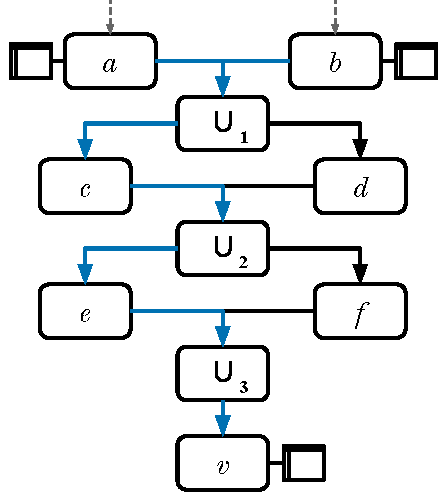
\includegraphics{diagrams/Chained Unions.pdf}
  \caption{Chained unions. Only nodes $a$, $b$, and $v$ hold state. Highlighted
  in \textbf{\color{brewerorange}orange} are two upquery paths that $\cup_1$
  must combine upquery responses for.}
  \label{f:chained-union}
\end{figure}

Figure~\vref{f:chained-union} shows a dataflow segment where the precise grouping
mechanism is important (\texttt{upquery\_path\_group} in the code listing).
There are three unions in a chain, which makes eight distinct upquery paths. If
$v$ encounters missing state, it must therefore issue eight upqueries, one for
each path. $a$ and $b$ both appear as the root of four paths, and will be
upqueried that many times. The issue arises at the unions, which need to do
the aforementioned union buffering.

Ultimately, a single upquery response must reach $v$. This means that $\cup_3$
must receive two upquery responses, one from $e$ and one from $f$, which it must
then combine. So $\cup_2$ must \emph{produce} two upquery responses, one
destined for $e$ and one for $f$. This in turn means that $\cup_2$ must receive
two upquery responses from $c$, and two from $d$. Which again means that
$\cup_1$ must produce four responses, two for $c$ and two for $d$, out of the
eight responses it receives (four from $a$ and four from $b$).

These are all the upqueries that pass through $\cup_1$:
        
\begin{multicols}{4}
\begin{description}
  \item [1.] $a\,\to\,c\,\to\,e$
  \item [2.] $a\,\to\,c\,\to\,f$
  \item [3.] $a\,\to\,d\,\to\,e$
  \item [4.] $a\,\to\,d\,\to\,f$
  \item [5.] $b\,\to\,c\,\to\,e$
  \item [6.] $b\,\to\,c\,\to\,f$
  \item [7.] $b\,\to\,d\,\to\,e$
  \item [8.] $b\,\to\,d\,\to\,f$
\end{description}
\end{multicols}

$\cup_1$ must combine these in pairs such that every downstream union receives
the responses that they expect from each of their inputs. The grouping that
achieves this is:

\begin{multicols}{2}
\begin{description}
  \item [1/5.] $a/b\,\to\,c\,\to\,e$
  \item [2/6.] $a/b\,\to\,c\,\to\,f$
  \item [3/7.] $a/b\,\to\,d\,\to\,e$
  \item [4/8.] $a/b\,\to\,d\,\to\,f$
\end{description}
\end{multicols}

The key observation is that the distinction between $a$ and $b$ does not matter
any longer downstream of $\cup_1$; a delta that arrived from $a$ is
indistinguishable from one that arrived from $b$. Similarly, the distinction
between $c$ and $d$ no longer matters past $\cup_2$, and the same for $e$ and
$f$ past $\cup_3$. \texttt{upquery\_path\_group} is thus defined as a unique
identifier for $v$'s upquery plan plus the sequence of nodes between the union
and the target of the upquery response.

\subsection{Joins}

For unions the upquery must go to all the ancestors. For joins on the other
hand, the upquery must only go to \textbf{one} ancestor. This is because when a
join processes a message from one ancestor, it already queries the ``other''
ancestor and thus pulls in any relevant state. If both sides of the join were
queried, the processing of the upquery responses at the join would produce
duplicates of every record.

Noria supports two types of joins: inner joins and partial outer joins (i.e.
``left'' and ``right'' joins). For an inner join, either ancestor can be the
target of the upquery, whereas for a partial outer join, the upquery \emph{must}
go to the ``full'' side\,---\,the side from which all rows are
yielded\footnote{An upquery for a column that originates from the non-full
ancestor must be routed according to its value. If it is \texttt{NULL}, the
upquery must go to the left, with additional later filtering, whereas if it is
non-\texttt{NULL}, it can go to the non-full side without issue. Noria does not
support such upqueries.}. Otherwise, the upquery may produce only a subset of
the results for the join.

\subsubsection{Dependent Upqueries}

Since upqueries travel through only one ancestor of a join, joins do not need to
buffer upquery responses the same way unions do. However, when a upquery
response passes through a join operator, the join does perform lookups into the
state of the other side of the join. With partial state, those lookups may
themselves encounter missing entries. When this happens, a problem arises: Noria
\emph{must} produce an downstream upquery response because the application is
waiting for it, but cannot produce that response since required state is
missing.

For the purposes of exposition, and without loss of generality, the text below
refers to the join ancestor that was upqueried as the left side, and the
ancestor that a lookup missed in as the right side.

The join must issue an upquery to the right hand side for the state that is
missing to complete the processing of the original upquery response from the
left. However, this \textit{dependent upquery} may take some time to complete,
and the system must decide what to do in the meantime. Recall that the join is
still in the middle of processing an upquery response.

An obvious, but flawed strategy is to have the join block until the response
arrives. This would not only stall processing of deltas from the left parent,
but also leads to a deadlock. In order to observe the eventual upquery response,
the join's domain must continue to process incoming messages to the right parent
(\S\ref{s:join-state-dupe}). But in doing so, it may encounter a different
upquery response from the right parent. That upquery response may require a
lookup into the left parent's state, which may itself encounter missing entries.
The join is then forced to block on both inputs perpetually.

Instead, the join \emph{discards} the current upquery response, and notes down
the upquery parameters that triggered it, and the missing state it is waiting to
be filled. It then continues processing the next update as normal. When all the
missing entries are eventually filled in, the system \emph{re-issues} the
original upquery to the join's left parent using the parameters it saved. This
time, when the upquery response arrives, all entries required for the lookups
into the right-hand parent's state should be present, and the downstream upquery
response is produced. As far as the downstream dataflow is concerned, nothing
abnormal has happened\,---\,the upquery response just took longer to arrive.

\subsubsection{Incongruent Joins}
\label{join-evictions}

As discussed in \S\ref{s:partial:linear}, if some key $k$ is present in a
materialization $m$, it must also be present at every materialization above $m$
from the upquery chain that ultimately produced the entry for $k$ in $m$.
However, certain query graphs produce dataflow where more than one key is used
in the dataflow to compute an entry. Consider a dataflow that joins two inputs,
\texttt{story} and \texttt{user}, on the story's author field. A downstream
operator issues an upquery for story number 7. The upquery is issued to
\texttt{story}, which produces a message that contains story number 7 with
author ``Elena''. That message arrives at the join, which issues a dependent
upquery to \texttt{user} for ``Elena''. When that dependent upquery resolves,
the join produces the final upquery response, and the state for story number 7
is populated in the downstream materialization.

Next, an editor changes the author for story number 7 to ``Talia''. This
takes the form of a delta with a negative multiplicity record for \texttt{[7,
"Elena"]} and a positive one for \texttt{[7, "Talia"]}. When this delta arrives
at the join, it may now miss when performing the lookup for ``Talia''. According
to the partial model so far, the join should drop \texttt{[7, "Talia"]}, and
only allow the negative for ``Elena'' to propagate to the downstream
materialization. But this violates Invariant~\ref{i:missing-suffix}, since there
exists downstream state that reflects the discarded update. And indeed, when
this happens, the state for article number 7 becomes empty (though not missing),
and any subsequent read for article number 7 receives an empty response, which
violates Invariant~\ref{i:prefix-consistency}.

What happened here was that the entry for key $k$ in the leaf-most
materialization depends not only on state entries indexed by the same $k$
upstream, but also on state entries indexed by other keys upstream. While $k$
must be present upstream, no such guarantee exists for other keys.

This is a result of \textit{incongruent joins}; joins whose join column is not
the same as the downstream key column. Incongruence is determined with respect
to each upquery path that flow through a join. In the case above, the author
join is incongruent with an upquery on the story number column, since the join
column is the author column. However, the join is congruent with upqueries from
a hypothetical downstream view that is keyed by author instead. A join that is
incongruent with any upquery path that flows through it is considered an
incongruent join.

Noria can easily recognize incongruent joins through key provenance
analysis\,---\,if an upquery flows through a join, and the upquery column is not
the same as the join column, the join is incongruent. If an incongruent join
encounters missing state while processing a delta at runtime, it must take
action to ensure that downstream state remains correct. Since the domain that
processes the join cannot produce a valid delta, and does not know what state is
present and missing in the downstream dataflow, its only option is to issue an
eviction for any downstream state that \emph{may} be rendered stale. Concretely,
if an incongruent join processes a record $r$ and encounters a missing state
entry, it should issue an eviction downstream on all incongruent upquery paths
using the appropriate values from $r$. For example, if the join column is $c_j$,
and upquery path $u_i$ through the join is keyed by column $c_i$, then the join
should issue downstream evictions of $r[c_i]$ for each $u_i$ where $c_i \neq
c_j$.

\paragraph{All Together Now.}
%
With unions and joins covered, the argument is complete. In all dataflows that
Noria can construct, no matter how they diverge and merge, the outlined
mechanisms ensure that the system invariants are maintained at every node, and
thus in Noria as a whole.

\section{Sharding}
\label{s:challenge:sharding}

Noria supports sharding cliques of operators to increase the throughput of
particular sections of the dataflow (\S\ref{s:noria:sharding}). And upqueries
must also work Noria decides to shard operators in this way. Partial state with
sharding mainly follows the rules of partial across unions
(\S\ref{s:upqueries:union}), with the following three modifications:

First, if the node that receives the upquery, R, is sharded the same way as the
querying node, Q, the upquery is sent \emph{only} to the same shard of R as the
one that is querying. This is called a \textit{narrow} upquery, and avoids
queries to shards that hold no relevant data. This rule applies even if the
upquery key differs from the sharding key, since while other shards may have
relevant data, that data would be discarded before reaching the current node
anyway. Noria decides whether upqueries should be narrow or broad when it
determines an operator's upquery plan\,---\,key provenance provides sufficient
information to make the decision.

Second, when a narrow upquery response reaches the \emph{first} shard merger
(effectively a union across shards) on its path, the response must not be
buffered, unlike other upquery responses across unions. This is because
the other upstream shards will not be sending responses.

Third, when the upquery response for an upquery that originated at a sharded
node reaches the \emph{last} sharder on its path, that sharder must direct that
response only to the querying shard. This is equivalent to the general rule that
upquery responses only flow along the edges that the upquery traversed. The
upquery that triggered the response did not touch other shards of the upquery
originator, and so the response should not go there.

Beyond those three modifications, the existing logic for handling upqueries
across forked strands of dataflow is sufficient.

% \footnote{Since shard mergers have only one operator (but many shards) as their
% ancestor, they use the shard index of the operator that sent each input as a way
% to distinguish between input paths, rather than the index of the operator
% itself. Otherwise, they operate entirely as a union.}
